\documentclass[11pt]{article}

\usepackage[T1]{fontenc}
\usepackage[utf8]{inputenc}
\usepackage[a4paper,margin=28mm]{geometry}
\usepackage{amsmath,amssymb,mathtools}
\usepackage{booktabs}
\usepackage{tabularx}
\usepackage{graphicx}
\usepackage{microtype}
\usepackage{natbib}
\usepackage{siunitx}
\usepackage{xurl}
\usepackage[hidelinks]{hyperref}
\usepackage[nameinlink,noabbrev]{cleveref}
\usepackage{xcolor}

\crefname{equation}{equation}{equations}
\Crefname{equation}{Equation}{Equations}
\crefname{figure}{figure}{figures}
\Crefname{figure}{Figure}{Figures}
\crefname{table}{table}{tables}
\Crefname{table}{Table}{Tables}
\crefname{section}{section}{sections}
\Crefname{section}{Section}{Sections}

\newcommand{\Na}{\mathrm{Na}^{+}}
\newcommand{\K}{\mathrm{K}^{+}}
\newcommand{\Cl}{\mathrm{Cl}^{-}}
\newcommand{\HCO}{\mathrm{HCO}_{3}^{-}}
\newcommand{\COthree}{\mathrm{CO}_{3}^{2-}}
\newcommand{\Ca}{\mathrm{Ca}^{2+}}
\newcommand{\Ae}{\mathrm{AE4}}
\newcommand{\NKCC}{\mathrm{NKCC1}}
\newcommand{\NHE}{\mathrm{NHE1}}
\newcommand{\NBC}{\mathrm{NBC}}
\newcommand{\CaCC}{\mathrm{CaCC}}
\newcommand{\TIC}{\mathrm{TIC}}
\newcommand{\TA}{\mathrm{TA}}
\newcommand{\dd}{\mathrm{d}}

\title{AE4 control of salivary secretion nearly a decade later: chloride availability, conservation and the limits of transporter compensation}

% TODO: confirm the complete author list, order and affiliations with all contributors.
\author{Elías Vera-Sigüenza}
\date{Revised manuscript, 18 September 2026}

\begin{document}
\maketitle

\begin{abstract}
AE4 deletion impairs salivary secretion despite the presence of other chloride uptake pathways. Our 2018 model attributed this dependence to the cation coupling of AE4. Here we reassess that explanation using an acinar model with explicit ion amounts, inorganic carbon, alkalinity, finite buffering, water transport and electrical closure. Reconstruction exposes two distinct issues. Productive AE4 chloride loading requires adequate alkalinity supply under the specified transporter constraints, whereas state dependent NKCC1 compensation can almost erase the secretion phenotype. Equal sodium and potassium routing gives only a 3.86\% cumulative deficit in that compensating network. A predeclared panel of seven source classes motivated by Catalán et al. (2025) produces small or reversed effects, or fails physiological pH checks, when coupled to the inherited kinetic law. A separate phenotype calibrated apical coupling produces a 30.26\% deficit but does not identify a molecular mechanism.

The final comparison instead asks whether chloride availability can create AE4 dependence under shared secretory demand. Measured wild type and knockout chloride and pH values define projected onset states; non-AE4 chloride supply is matched as an explicit model idealisation. Without an AE4 specific channel multiplier, knockout cumulative secretion is 20.04--20.10\% lower across three shared auxiliary chloride conductances. An exact chloride balance accounts for the additional wild type apical export through the initial reservoir advantage, continuing AE4 supply and the remaining intracellular difference, closing within $7.5\times10^{-8}$ fmol at 600 s. The result supports a conditional chloride availability mechanism, rather than identifying cation routing or direct channel recruitment as the sole cause. Catalán et al. (2015) motivate a shared beta adrenergic secretory pathway; the 2025 molecular findings constrain AE4 transport without fixing its whole cell kinetics. The remaining limitations concern onset and supply assumptions and stimulus specificity, not failure to equal one experimental percentage.
\end{abstract}

\noindent\textbf{Keywords:} salivary secretion; AE4; SLC4A9; chloride reservoir; alkalinity; NKCC1; mathematical physiology

\section{Introduction}
\label{sec:introduction}

Acinar fluid secretion depends on the accumulation of intracellular chloride, its release across the apical membrane, and the accompanying movement of cations and water. This physical description is simple; determining which transporters make secretion sensitive to a particular gene deletion is not. A pathway can carry an appreciable fraction of the normal chloride load yet have little effect on secretion after its removal if another pathway compensates. Conversely, a transporter can matter because it establishes the ionic state from which secretion begins, rather than because its instantaneous flux is uniquely indispensable \citep{Melvin2005,Gin2007,Palk2010}.

The model considered here describes the acinar stage of secretion. Acini generate primary fluid and electrolytes; the ducts subsequently modify the ionic composition of saliva \citep{thaysen1954excretion,young1966micropuncture}. We compare relative changes in acinar outflow with the whole gland phenotype, but do not equate the output of one model cell with absolute gland flow or represent ductal transport explicitly.

NKCC1 supplies the dominant basolateral chloride uptake route, while bicarbonate dependent exchange provides a parallel contribution \citep{martinez1983effect,evans2000severe,nguyen2004cl}. In mouse submandibular glands, \citet{Pena2015} found that AE4 deletion reduced total secretion during combined carbachol (CCh) and isoproterenol (IPR) stimulation by approximately $35\pm4.7\%$, whereas AE2 deletion had little effect. Resting intracellular chloride was $50.10\pm1.50$ mM in wild type and $36.50\pm1.60$ mM in AE4 knockout, despite similar resting pH. Chloride uptake was selectively impaired in beta containing protocols, while the CCh only uptake response was comparatively preserved. The isolated NKCC assay showed no statistically detectable genotype difference. These observations constrain different aspects of the mechanism; none can be replaced by a requirement to reproduce exactly 35\% at a chosen instant.

Our original model reproduced an approximately 24\% reduction after AE4 loss and a negligible AE2 effect \citep{VeraSiguenza2018}. It attributed the distinction to monovalent cation coupling: AE4 removal increased intracellular sodium and potassium, altered NHE1 and pump activity, and reduced chloride accumulation. NKCC1 activation after exchanger loss was small in that model. Its acid--base system explicitly represented bicarbonate, protons and carbon dioxide, but contained no additional bicarbonate uptake transporter. Sodium and potassium transport through AE4 was allocated according to their intracellular abundance. The original result therefore demonstrated a possible explanation within a particular transport network; agreement with a secretion deficit did not establish that explanation as unique.

Two strands of subsequent evidence sharpen the question. First, AE4 is an electroneutral, monovalent cation dependent chloride--bicarbonate exchanger, with both sodium and potassium supporting transport \citep{Pena2016}. Beta stimulation activates AE4 through cAMP/PKA and depends on its S173 region \citep{Pena2021}. These findings support regulated chloride loading, but do not determine an acute signalling time constant or a complete native acinar kinetic law. In human AE4, \citet{Catalan2025} identified residues contributing to bicarbonate and cation coordination. In particular, the T448I/T756A double mutant lost sodium supported transport while retaining potassium supported activity. These are molecular constraints, not a direct measurement of a unique whole transport cycle in the mouse gland.

Second, the apical demand side is more diverse than a single muscarinic chloride channel. \citet{Catalan2015} showed that acinar TMEM16A deletion abolished calcium dependent secretion while leaving an IPR response. Pharmacological inhibition and the associated swelling and anion current implicated a distinct volume sensitive pathway. This does not establish that AE4 specifically recruits that channel. An alternative is that a pathway shared by both genotypes exposes different intracellular chloride availability.

We accordingly distinguish three questions. Can a conservation based reconstruction support productive AE4 transport while maintaining acid--base balance? Does removing that transport necessarily reduce secretion once compensating pathways respond? Finally, can the measured chloride difference, together with continuing wild type AE4 supply, produce a substantial deficit under shared secretory demand? The first two questions expose weaknesses in seemingly plausible mechanisms. The third changes the comparison from acute removal at a common wild type state to a conditional comparison informed by the established genotype states.

The manuscript follows the scientific argument rather than the order of implementation. We retain the negative results because they identify where a plausible explanation becomes misleading: charge balance without adequate alkalinity supply, compensation inferred from an unsuitable assay mapping, proposed source stoichiometry combined with incompatible kinetics, initiation confused with parameter identification, and phenotype calibration presented as validation. The final reservoir comparison is a demonstration under explicit onset and supply assumptions. It is not an independently identified chronic knockout model and is not made valid or invalid by its distance from a single experimental mean.

\section{Model}
\label{sec:model}

The reconstructed model describes one acinar cell, a finite luminal compartment and an infinite extracellular bath. It retains the well-stirred approximation used in the original AE4 model, but replaces several concentration equations by conserved amount balances. This change is essential for acid--base chemistry, because internal protonation reactions may redistribute carbon species without creating carbon or alkalinity. The historical compensating network and the final prescribed-supply comparison share these conservation equations, but not every constitutive assumption.

\subsection{Compartments, amounts and concentrations}

Let $n_{s,i}$ and $n_{s,l}$ denote the intracellular and luminal amounts of ion $s\in\{\Na,\K,\Cl\}$. The cell and lumen volumes are $V_i$ and $V_l$, and concentrations are obtained from
\begin{equation}
    [s]_r=\frac{n_{s,r}}{V_r}, \qquad r\in\{i,l\}.
    \label{eq:amount-concentration}
\end{equation}
The numerical units are fmol for amount, pL for volume and mM for concentration, so the conversion in \cref{eq:amount-concentration} is exact. The bath concentrations remain constant.

Rather than evolve free bicarbonate and proton concentrations independently, we evolve the total inorganic carbon amount $n_{T,r}$ and total alkalinity amount $n_{A,r}$ in each finite compartment. The complete core state is therefore
\begin{equation}
\begin{aligned}
    y={}&(n_{\mathrm{Na},i},n_{\mathrm{K},i},n_{\mathrm{Cl},i},n_{T,i},n_{A,i},V_i,\\
       &n_{\mathrm{Na},l},n_{\mathrm{K},l},n_{\mathrm{Cl},l},n_{T,l},n_{A,l},V_l),
\end{aligned}
\label{eq:state-vector}
\end{equation}
augmented by one inherited AE4 regulatory coordinate per cell, giving 13 states per genotype. This amount formulation makes dilution, charge accounting and water transport explicit.

\subsection{Carbonate chemistry and intracellular pH}
\label{sec:acid-base}

Total inorganic carbon is the sum of dissolved carbon dioxide, bicarbonate and carbonate,
\begin{equation*}
    T=[\mathrm{CO}_2]+[\HCO]+[\COthree].
\end{equation*}
We include one finite monoprotic non-carbonate buffer with total concentration $B_T=[\mathrm{BH}]+[\mathrm{B}^{-}]$. Total alkalinity is
\begin{equation}
    A=[\HCO]+2[\COthree]+[\mathrm{B}^{-}]+[\mathrm{OH}^{-}]-[\mathrm{H}^{+}].
    \label{eq:total-alkalinity}
\end{equation}
For fixed $T$, $A$, $B_T$ and volume, pH is recovered by solving \cref{eq:total-alkalinity} together with the two carbonate dissociation equilibria, water ionisation and the buffer equilibrium. If $K_1$, $K_2$ and $H=[\mathrm H^+]$ denote the carbonate equilibrium constants and proton concentration, the carbon fractions are
\begin{align*}
    \alpha_{\mathrm{CO}_2}&=\frac{H^2}{H^2+K_1H+K_1K_2},\\
    \alpha_{\HCO}&=\frac{K_1H}{H^2+K_1H+K_1K_2},\\
    \alpha_{\COthree}&=\frac{K_1K_2}{H^2+K_1H+K_1K_2}.
\end{align*}
Thus $[\mathrm{CO}_2]=T\alpha_{\mathrm{CO}_2}$, $[\HCO]=T\alpha_{\HCO}$ and $[\COthree]=T\alpha_{\COthree}$. Fast internal hydration and protonation reactions conserve both $T$ and $A$. External species fluxes are mapped to these coordinates. One bicarbonate adds one unit of carbon and one equivalent of alkalinity, one carbonate adds one unit of carbon and two equivalents of alkalinity, and proton extrusion raises alkalinity by one equivalent.

This formulation is the first material departure from the 2018 acid--base model. There, carbon dioxide hydration produced free bicarbonate and protons, NHE1 removed protons, and AE2 and AE4 exported bicarbonate. No additional bicarbonate uptake pathway was present \citep{VeraSiguenza2018}. In the present model, the same biological processes are retained but their effects are expressed in conserved coordinates, which reveals directly whether a proposed transporter can support sustained AE4 activity without violating alkalinity balance.

\subsection{Whole-cell amount balances}

We use positive fluxes in the directions specified below. $J_N$ is the inward NKCC1 cycle flux, $J_H$ is the inward-sodium/outward-proton NHE1 flux, $J_2$ is the inward-chloride/outward-bicarbonate AE2 flux, $J_B$ is the inward electrogenic NBC cycle flux, and $S^4_s$ is the AE4 source for species or conserved quantity $s$. $P_a$ and $P_b$ are apical and basolateral sodium--potassium pump cycle rates. $J_{K,a}$ and $J_{K,b}$ are potassium effluxes from cell to lumen and bath, and $J_{Cl,a}$ is apical chloride efflux. With these conventions, the intracellular balances are
\begin{equation}
\begin{aligned}
\dot n_{\mathrm{Na},i}={}&J_N+J_H+J_B+S^4_{\mathrm{Na}}-3(P_a+P_b),\\
\dot n_{\mathrm{K},i}={}&J_N+S^4_{\mathrm K}+2(P_a+P_b)-J_{K,a}-J_{K,b},\\
\dot n_{\mathrm{Cl},i}={}&2J_N+J_2+S^4_{\mathrm{Cl}}-J_{Cl,a},\\
\dot n_{T,i}={}&J_{\mathrm{CO}_2,b}+J_{\mathrm{CO}_2,a}-J_2+S^4_T+2J_B,\\
\dot n_{A,i}={}&J_H-J_2+S^4_A+2J_B,\\
\dot V_i={}&q_b-q_a.
\end{aligned}
\label{eq:cell-balances}
\end{equation}
Here $J_{\mathrm{CO}_2,b}$ is carbon dioxide transport from bath to cell and $J_{\mathrm{CO}_2,a}$ is transport from lumen to cell. The corresponding luminal balances are
\begin{equation}
\begin{aligned}
\dot n_{\mathrm{Na},l}={}&3P_a-J^p_{\mathrm{Na}}-q_{\mathrm{out}}[\Na]_l,\\
\dot n_{\mathrm{K},l}={}&-2P_a+J_{K,a}-J^p_{\mathrm K}-q_{\mathrm{out}}[\K]_l,\\
\dot n_{\mathrm{Cl},l}={}&J_{Cl,a}-J^p_{\mathrm{Cl}}-q_{\mathrm{out}}[\Cl]_l,\\
\dot n_{T,l}={}&-J^p_{\HCO}-J_{\mathrm{CO}_2,a}-q_{\mathrm{out}}T_l,\\
\dot n_{A,l}={}&-J^p_{\HCO}-q_{\mathrm{out}}A_l,\\
\dot V_l={}&q_a+q_t-q_{\mathrm{out}}.
\end{aligned}
\label{eq:lumen-balances}
\end{equation}
The paracellular fluxes $J^p_s$ are positive from lumen to bath. The lumen is finite, and therefore secretion removes both water and dissolved solutes through the outflow terms in \cref{eq:lumen-balances}.

\subsection{Basolateral chloride loading and pH regulation}

\subsubsection{NKCC1}

NKCC1 transports one sodium, one potassium and two chloride ions per inward cycle. The final reservoir construction retains the earlier reversible phenomenological law
\begin{equation}
 J_N^{\rm local}=m_N G_N\tanh(A_N/w_N),\qquad
 A_N=\log\frac{[\Na]_e[\K]_e[\Cl]_e^2}{[\Na]_i[\K]_i[\Cl]_i^2}.
 \label{eq:nkcc-prepalk}
\end{equation}
The historical Palk/Benjamin comparison instead used the reduced concentration response \citep{Benjamin1997,Palk2010}
\begin{equation}
 J_N=\alpha_N m_N
 \frac{a_1-a_2[\Na]_i[\K]_i[\Cl]_i^2}
      {a_3+a_4[\Na]_i[\K]_i[\Cl]_i^2}.
 \label{eq:nkcc1}
\end{equation}
Its prefactor is fixed from the accepted wild type rest, with algebraic activity $m_N=1$ at rest and 1.75 at full muscarinic activation. This gain is an inherited effective construction, not a universal physiological constant. The reduced law in \cref{eq:nkcc1} does not describe extracellular chloride depletion and readdition faithfully. Its genotype response during normal model stimulation must therefore not be equated with the isolated NKCC assay. The final comparison deliberately excludes this later module and prescribes paired supply as described in \cref{sec:reservoir-comparison}.

\subsubsection{NHE1}

NHE1 exchanges one extracellular sodium for one intracellular proton. We use the eight-state reduction of \citet{Cha2009}. Let
\begin{align*}
 a&=k_1^+\frac{[\Na]_e}{[\Na]_e+K_{Na,o}}
       \frac{K_{H,o}}{[\mathrm H^+]_e+K_{H,o}},\\
 b&=k_2^+\frac{[\mathrm H^+]_i}{[\mathrm H^+]_i+K_{H,i}}
       \frac{K_{Na,i}}{[\Na]_i+K_{Na,i}},\\
 c&=k_1^-\frac{[\Na]_i}{[\Na]_i+K_{Na,i}}
       \frac{K_{H,i}}{[\mathrm H^+]_i+K_{H,i}},\\
 d&=k_2^-\frac{[\mathrm H^+]_e}{[\mathrm H^+]_e+K_{H,o}}
       \frac{K_{Na,o}}{[\Na]_e+K_{Na,o}}.
\end{align*}
The exchanger flux is
\begin{equation}
    J_H=N_H m_H(t) M_2\frac{ab-cd}{a+b+c+d},
    \qquad
    M_2=\left[1+\left(1+\frac{[\mathrm H^+]_e}{K_{M,o}}\right)
    \left(\frac{K_{M,i}}{[\mathrm H^+]_i}\right)^3\right]^{-1}.
    \label{eq:nhe1}
\end{equation}
$N_H$ is the wild-type carrier amount obtained from the resting pH reconstruction, while $m_H(t)$ rises from one at rest to 2.3 under full stimulation. One positive cycle adds one sodium amount and one alkalinity equivalent to the cell.

\subsubsection{AE2}

AE2 is represented by a reversible chloride--bicarbonate exchange law,
\begin{equation*}
    J_2=G_2\tanh\!\left(\frac{A_2}{w}\right),
    \qquad
    A_2=\log\!\left(\frac{[\Cl]_e[\HCO]_i}{[\Cl]_i[\HCO]_e}\right),
\end{equation*}
where positive flux imports chloride and exports bicarbonate. It contributes $+J_2$ to intracellular chloride and $-J_2$ to both TIC and TA.

\subsubsection{Stimulus-recruited sodium--bicarbonate cotransport}
\label{sec:nbc}

The reconstructed model includes a minimal electrogenic NBC-like pathway,
\begin{equation*}
    [\Na]_e+2[\HCO]_e \rightleftharpoons [\Na]_i+2[\HCO]_i.
\end{equation*}
This is a structural pathway rather than an assignment to a particular salivary SLC4 isoform. Its inward affinity and flux are
\begin{equation}
\begin{aligned}
    A_B&=\log\!\left(
       \frac{[\Na]_e[\HCO]_e^2}{[\Na]_i[\HCO]_i^2}
       \right)+\frac{V_b}{V_T},\\
    J_B&=u(t)G_B\tanh\!\left(\frac{A_B}{w_B}\right).
\end{aligned}
\label{eq:nbc}
\end{equation}
Here $V_T=RT/F$, and $V_b=\phi_i-\phi_e$ is the basolateral potential. The activation $u(t)$ is exactly zero at the resting calcium concentration and one at the standard stimulated calcium input. Thus the accepted resting model is an exact nesting limit. Each inward cycle adds one sodium amount, two units of TIC and two alkalinity equivalents. It carries one net negative charge into the cell, so the conventional current is $I_B=FJ_B$ in the cell-to-bath current convention and is included in basolateral current closure.

The role of this pathway can be read directly from \cref{eq:cell-balances}, conditional on the other transport capacities and state constraints. Without NBC, the sustained alkalinity balance is
\begin{equation*}
    0=J_H-J_2+S_A^4.
\end{equation*}
For the original AE4 stoichiometry, $S_A^4=-2J_4$. Substantial AE4 chloride loading therefore requires either a comparably large NHE1 flux or another inward source of alkalinity. In the frozen reconstruction, the permitted NHE1 response was too small to support the declared productive AE4 load at an acceptable state. This is not a general proof that an NBC isoform is the only possible biological source of alkalinity. With NBC, the sustained balance becomes
\begin{equation}
    0=J_H+2J_B-J_2+S_A^4,
    \label{eq:alkalinity-balance}
\end{equation}
which provides an additional alkalinity source without importing chloride directly. Zero resting recruitment is an exact nesting choice, not evidence that native basal bicarbonate cotransport is absent.

\subsection{AE4 transport and regulation}

The parent AE4 flux is a reversible two-conformation, shared-carrier quasi-steady model. It has one common chloride transition and separate sodium- and potassium-loaded return transitions. For cation $c\in\{\Na,\K\}$, the forward affinity of the original $1\Cl:1c:2\HCO$ cycle is
\begin{equation}
    A_{4,c}=\log\!\left(\frac{[\Cl]_e}{[\Cl]_i}\right)
           +\log\!\left(\frac{[c]_i}{[c]_e}\right)
           +2\log\!\left(\frac{[\HCO]_i}{[\HCO]_e}\right).
    \label{eq:ae4-affinity}
\end{equation}
The effective forward and reverse rates are constructed symmetrically, $k^+=\bar k\exp(A/2)$ and $k^-=\bar k\exp(-A/2)$, so local detailed balance and the exact reversal condition are preserved. If $p_o$ and $p_i$ are the two carrier occupancies, the cation branch fluxes are
\begin{align*}
    J_{4,\Na}&=N_4m_4(t)(k_{\Na}^{+}p_i-k_{\Na}^{-}p_o),\\
    J_{4,\K}&=N_4m_4(t)(k_{\K}^{+}p_i-k_{\K}^{-}p_o),
\end{align*}
and the total chloride-loading cycle is $J_4=J_{4,\Na}+J_{4,\K}$.

Beta-adrenergic regulation is represented by one effective activation fraction $x_4$,
\begin{equation}
    \dot x_4=\frac{\beta(t)-x_4}{\tau_4},
    \qquad m_4(t)=1+g_4x_4,
    \label{eq:ae4-regulation}
\end{equation}
with $\tau_4=30$ s and $g_4=0.25$. The existence and direction of beta/cAMP/PKA regulation are source supported \citep{Pena2021}, but the 30 s filter and the selected gain are inherited model assumptions. They are retained unchanged, not identified from an experimental timing target.

The final reservoir model retains the donor weighted allocation of its earlier parent. With $f_d=[\Na]_d/([\Na]_d+[\K]_d)$, where the donor is intracellular for $J_4\geq0$ and extracellular for $J_4<0$, its source is
\begin{equation}
 (S^4_{\rm Na},S^4_{\rm K},S^4_{\rm Cl},S^4_T,S^4_A)
 =(-f_d,-(1-f_d),1,-2,-2)J_4.
 \label{eq:donor-routing}
\end{equation}
This is an effective allocation of the inherited scalar cycle, not a measurement of microscopic sodium and potassium stoichiometry. In particular, retaining a reversible scalar carrier law does not independently validate every effective source allocation attached to it.

For the equal-routing model, the total scalar cycle $J_4$ is retained but its cation source is divided equally between sodium and potassium. The conserved-coordinate source is
\begin{equation}
    \left(S^4_{\mathrm{Na}},S^4_{\mathrm K},S^4_{\mathrm{Cl}},S^4_T,S^4_A\right)
    =\left(-\tfrac12,-\tfrac12,1,-2,-2\right)J_4.
    \label{eq:equal-routing-source}
\end{equation}
This modification isolates cation routing from total AE4 chloride loading. It is not claimed to be a microscopic AE4 mechanism.

\subsection{Catalán 2025 mechanism classes}
\label{sec:catalan-classes}

Catalán et al. experimentally constrained the residues and cation dependence of human AE4, and proposed several possible electroneutral transport cycles \citep{Catalan2025}. The exact stoichiometries remain hypotheses. We therefore test a finite panel by keeping the inherited scalar $J_4(y,t)$ fixed and changing only the transported source vector. This first-stage construction asks what the proposed stoichiometries do to the whole-cell balances; it does not replace the missing class-specific kinetic law.

\begin{table}[t]
\centering
\caption{Predeclared AE4 source classes. Each row gives $(S_{\mathrm{Na}}^4,S_{\mathrm K}^4,S_{\mathrm{Cl}}^4,S_T^4,S_A^4)/J_4$.}
\label{tab:mechanism-classes}
\footnotesize
\begin{tabularx}{\textwidth}{lXXl}
\toprule
Class & Proposed cycle & Source vector & Reference affinity \\
\midrule
C0 & equal-routing $1:1:2$ control & $(-1/2,-1/2,1,-2,-2)$ & opposed \\
C1 & $\Cl+\Na$ in, $\K+\HCO$ out & $(1,-1,1,-1,-1)$ & supported \\
C2 & $\Cl+\Na$ in, $2\K+\COthree$ out & $(1,-2,1,-1,-2)$ & supported \\
C3a & $\Cl$ in, $\K+2\HCO$ out & $(0,-1,1,-2,-2)$ & supported \\
C3b & $\Cl$ in, $\Na+2\HCO$ out & $(-1,0,1,-2,-2)$ & opposed \\
C4a & $\Cl$ in, $\K+\COthree$ out & $(0,-1,1,-1,-2)$ & supported \\
C4b & $\Cl$ in, $\Na+\COthree$ out & $(-1,0,1,-1,-2)$ & opposed \\
\bottomrule
\end{tabularx}
\end{table}

The carbonate classes distinguish carbon from alkalinity: outward transport of one $\COthree$ removes one unit of TIC and two equivalents of TA. Representing carbonate as bicarbonate would therefore violate both the chemistry and charge balance. All seven source vectors in \cref{tab:mechanism-classes} are exactly electroneutral and change sign when $J_4$ reverses. The affinity labels refer only to the frozen reference state. Source electroneutrality and formal reversal do not establish agreement between the inherited scalar flux and the affinity of each proposed cycle. These classes are historical comparisons, not the definition of the final donor weighted model.

\subsection{Membrane currents and voltage closure}

The apical and basolateral membrane potentials are $V_a=\phi_i-\phi_l$ and $V_b=\phi_i-\phi_e$. The transepithelial potential is $V_t=V_b-V_a$. For ion $s$ of valence $z_s$, the Nernst potential between the named compartments is
\begin{equation*}
    E_s=\frac{V_T}{z_s}\log\!\left(\frac{[s]_{\mathrm{out}}}{[s]_{\mathrm{in}}}\right).
\end{equation*}
Calcium-activated potassium and chloride conductances use a Hill gate
\begin{equation*}
    h_{Ca}=\frac{[\Ca]_i^r}{[\Ca]_i^r+K_{Ca}^r},
\end{equation*}
and Ohmic currents $I=Gh_{Ca}(V-E)$. Total pump capacity is partitioned between apical and basolateral membranes. For either membrane side $r$,
\begin{equation*}
    P_r=P_{r,\max}
    \frac{[\Na]_i^3}{[\Na]_i^3+K_{Na}^3}
    \frac{[\K]_r^2}{[\K]_r^2+K_K^2}.
\end{equation*}
Each cycle exports three intracellular sodium ions and imports two potassium ions from the corresponding external compartment.

Paracellular currents are linear,
\begin{equation*}
    I_s^p=G_s^p(V_t-E_s^p),
\end{equation*}
with positive direction from lumen to bath. Membrane capacitance is fast relative to secretion, so voltages satisfy quasi-steady current closure,
\begin{equation}
\begin{aligned}
    I_a-I_p&=0,\\
    I_b+I_B+I_p&=0,
\end{aligned}
\label{eq:current-closure}
\end{equation}
where $I_B$ is omitted at rest because the NBC increment is then exactly zero. The voltage system is solved at every right-hand-side evaluation. Source-charge identities are checked independently against \cref{eq:current-closure}.

\subsection{Water transport and luminal outflow}

Water follows osmotic differences between the three compartments,
\begin{align*}
    q_b&=L_b(\Pi_i-\Pi_e), & q_a&=L_a(\Pi_l-\Pi_i),\\
    q_t&=L_t(\Pi_l-\Pi_e), & q_{\mathrm{out}}&=k_{\mathrm{out}}\max(V_l-V_{\mathrm{dead}},0).
\end{align*}
The osmolarities include sodium, potassium, chloride, total inorganic carbon and the fixed intracellular osmolyte pool. The resulting volume equations are already included in \cref{eq:cell-balances,eq:lumen-balances}. The outflow law is a finite-lumen compliance closure. It is used consistently across all comparisons and is not interpreted as an independently measured ductal pressure law.

\subsection{Final chloride reservoir comparison}
\label{sec:reservoir-comparison}

The final experiment uses the accepted pre-Palk model, including \cref{eq:nkcc-prepalk,eq:donor-routing}, without the phenotype calibrated apical coupling. Wild type has full AE4 expression and knockout has zero. The two cells evolve as a paired 26 dimensional system. In the central construction, the knockout receives the instantaneous signed wild type NKCC1 and AE2 cycle rates,
\begin{equation}
 J_N^{\rm KO}(t)=J_N^{\rm WT}(t),\qquad
 J_2^{\rm KO}(t)=J_2^{\rm WT}(t).
 \label{eq:matched-supply}
\end{equation}
Each imposed rate is applied through the complete electroneutral source vector, not through a chloride only correction. All other local fluxes, pH, volumes, membrane potentials and lumen states respond independently. The absence of a detectable genotype effect in the isolated uptake experiment motivates examining this construction; it does not establish \cref{eq:matched-supply} under physiological stimulation. Matched supply is therefore an explicit conditional model comparison, not an inferred native regulation law.

Both genotypes have the same auxiliary apical chloride conductance,
\begin{equation}
\begin{aligned}
 I_{\rm aux}&=\beta G_{\rm aux}(V_a-E_{\rm Cl}),\\
 G_{\rm aux}&\in\{0,2.32,4.49\}\ {\rm nS}.
\end{aligned}
 \label{eq:shared-demand}
\end{equation}
It enters the complete current closure together with TMEM16A. Positive outward chloride flux corresponds to $E_{\rm Cl}-V_a>0$. The three strengths are predeclared shared alternatives, not independently identified apical conductances obtained directly from a whole cell patch current. They test whether the result requires a specific auxiliary demand strength. No factor depending on AE4 expression multiplies either channel.

\subsubsection{Measured chloride and pH define onset, not chronic equilibria}

The imposed onset values are $[\Cl]_i=50.10$ mM and pH 6.91 for wild type, and $[\Cl]_i=36.50$ mM and pH 6.89 for knockout \citep{Pena2015}. Simply replacing chloride alone would violate charge and osmotic consistency. We therefore use a deterministic projection, without a transport solve or pre-stimulation relaxation.

Let $Q_f$ be the unchanged fixed anion equivalents, $B_f$ the finite buffer amount and $M_f$ the fixed osmotic amount including that buffer once. At imposed pH, define $a=\alpha_{\HCO}+2\alpha_{\COthree}$, $b=B_f/[1+10^{pK_B-\mathrm{pH}}]$ and $w=[\mathrm{OH}^-]-[\mathrm H^+]$. With bath osmolarity $O_e$, charge neutrality and isotonicity imply
\begin{align}
 O_e&=2[\Cl]_i+(1+a)T_i+w+(Q_f+b+M_f)/V_i,\\
 [\K]_i&=[\Cl]_i+aT_i+w+(Q_f+b)/V_i-[\Na]_i.
 \label{eq:onset-projection}
\end{align}
The central projection retains the parent sodium concentration and cell volume, solves the first equation for $T_i$, then the second for potassium. TA follows from the speciation formula. The lumen and regulatory coordinates remain unchanged. The alternate recorded projection retains sodium and TIC concentrations and solves instead for volume. Neither projection is a predicted genotype equilibrium.

The resulting central onset states are listed in \cref{tab:onset}. The sizeable TIC difference is a consequence of this assumption, not an additional measurement. It prevents interpreting this paired comparison as an isolated chloride perturbation with every other intracellular concentration held fixed.
\begin{table}[t]
\centering
\caption{Central projected onset states. Only chloride and pH are imposed from genotype measurements. Sodium and volume are inherited; potassium and TIC follow from the stated charge and osmotic projection.}
\label{tab:onset}
\begin{tabular}{lrr}
\toprule
Quantity & Wild type & AE4 knockout\\
\midrule
Intracellular chloride (mM) & 50.10 & 36.50\\
pH & 6.91 & 6.89\\
Intracellular sodium (mM) & 11.6361 & 11.6361\\
Intracellular potassium (mM) & 116.0230 & 114.8307\\
TIC concentration (mM) & 16.5973 & 31.3896\\
Cell volume (pL) & 1.448426 & 1.448426\\
\bottomrule
\end{tabular}
\end{table}

\subsubsection{An exact chloride budget}

Write $\delta(t)=n_{\rm Cl,i}^{\rm WT}(t)-n_{\rm Cl,i}^{\rm KO}(t)$ and
\begin{equation*}
 D_X(T)=\int_0^T\bigl(J_X^{\rm WT}(t)-J_X^{\rm KO}(t)\bigr)\,\dd t,
 \qquad X\in\{N,2,4\}.
\end{equation*}
Define $D_{Cl,a}$ analogously for the difference in total apical chloride export, including both channels. Subtracting and integrating the cell chloride equations gives
\begin{equation}
 D_{Cl,a}(T)=\delta(0)+2D_N(T)+D_2(T)+D_4(T)-\delta(T).
 \label{eq:reservoir-general}
\end{equation}
Under matched supply and complete knockout, this becomes
\begin{equation}
 D_{Cl,a}(T)=\delta(0)+\int_0^T J_4^{\rm WT}(t)\,\dd t-\delta(T).
 \label{eq:reservoir-matched}
\end{equation}
This identity is independent of the cation allocation. It separates initial chloride availability, continuing AE4 input and the chloride advantage remaining at the end. It does not assert that the initial reservoir is exhausted. Nor does it equate apical chloride export with fluid outflow: paracellular return, luminal accumulation and luminal concentrations remain in \cref{eq:lumen-balances}.

\subsection{Numerical protocol and evidence status}
\label{sec:numerics}

Combined CCh+IPR stimulation is applied for 600 s. Historical acute deletion comparisons start from their corresponding common frozen wild type rest; the final paired comparison instead uses \cref{tab:onset}. Calcium is prescribed and beta is an effective input, not a newly fitted signalling cascade. The final solver record uses Radau with relative tolerance $10^{-7}$, amount and regulatory absolute tolerances $10^{-10}$, volume tolerance $10^{-12}$ pL and maximum step 2 s. The continuous trajectory begins at $\epsilon=10^{-6}$ s from the unchanged onset state. The separate zero and right limit samples preserve the declared stimulus convention.

The numerical checks cover positivity, the inherited physiological domain, source charge, current closure, water and carbon accounting at accepted endpoints and integer second samples. A physiological failure ends a valid trajectory at its first detected failed sample. Passing these checks is not a proof of continuous time validity, asymptotic stability or chronic genotype consistency. No failed trace is extended to create a 600 s outcome.

Fluid and chloride headline integrals use the recorded one second trapezoidal rule, including the onset samples. The independent reservoir audit uses saved eight node Gauss--Legendre flux quadrature on each accepted integration step, with four node cross checks and a separately recorded onset contribution. Its absolute balance tolerance is $10^{-5}$ fmol and its quadrature comparison tolerance is $10^{-6}$ fmol. The coarser headline quadrature is not used to claim the tighter conservation accuracy.

All manuscript figures are time series derived from existing files. For the central cases, a file only check verifies trajectory hashes, state differences and reported integrals without importing a model or calling a solver. The additional supply, projection and agonist comparisons in \cref{tab:reported-sensitivities} are explicitly reported summary results; their raw trajectories are not available in this manuscript source snapshot. We retain their stated outcomes and limitations without fabricating curves or claiming a fresh numerical verification.

\section{Results}
\label{sec:results}

\subsection{Productive AE4 loading requires an explicit alkalinity budget}
\label{sec:wt-reconstruction}

The conserved formulation separates productive chloride uptake from the acid--base cost of producing it. For the effective $1\Cl:1$ cation:$2\HCO$ cycle, inward chloride transport through AE4 removes two alkalinity equivalents. Carbon dioxide hydration redistributes carbonate species but does not create alkalinity. The balance therefore constrains the combined contributions of NHE1, AE2 and bicarbonate cotransport, not AE4 in isolation.

With the frozen NHE1 response and the stimulus recruited NBC-like pathway, the accepted wild type reconstruction sustains productive AE4 loading while maintaining the sampled physiological state. Its pH ranges from 6.9100 to 7.0348 over the 600 s stimulus. In the saved 60--600 s positive chloride loading budget, NKCC1 supplies 79.9248\% and AE4 supplies 20.0752\%; AE2 has no positive contribution in that interval. The signed time series in \cref{fig:chloride-loading} show that AE2 is slightly outward, rather than absent. The partition establishes a substantial AE4 contribution within this model; it is not an exact quantitative match to every pharmacological estimate of NKCC1's share.

The result supports the additional alkalinity pathway under the specified architecture and capacities. It does not establish a particular salivary NBC isoform, prove that all alternative sources of alkalinity are impossible, or imply that zero basal cotransport is a biological fact. Those stronger conclusions would require a broader model class and independent measurements.

\begin{figure}[t]
\centering
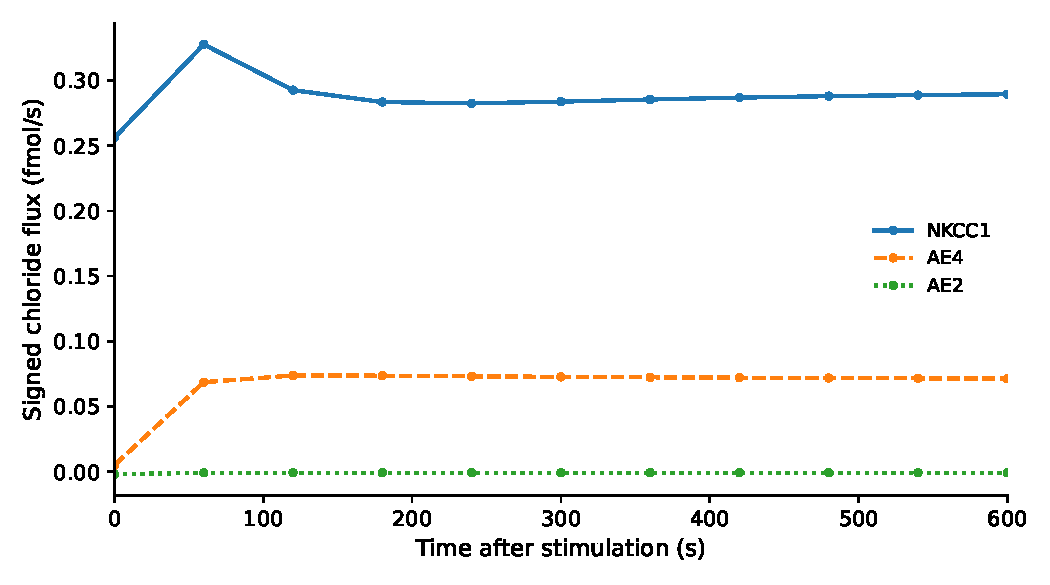
\includegraphics[width=\textwidth]{figures/fig01_chloride_loading.pdf}
\caption{Signed chloride loading in the accepted earlier wild type reconstruction. Points are the saved 60 s samples; joining segments do not resolve the early transient. NKCC1 and AE4 import chloride, while AE2 is slightly outward. The official 60--600 s positive loading fractions, 79.9248\% and 20.0752\%, are taken from the original integrated record, not recalculated from these coarse plotting samples.}
\label{fig:chloride-loading}
\end{figure}

\subsection{Later compensating networks conceal the effect of AE4 loss}
\label{sec:compensation}

Replacing the earlier NKCC representation by the Palk/Benjamin response produced strong compensation after acute AE4 removal. With donor weighted AE4 routing, the saved null trajectory increased integrated NKCC chloride loading by 33.10\% and reduced cumulative fluid secretion by only 0.627\%. Replacing the donor allocation by equal sodium and potassium routing reduced that compensation to 23.16\%, but the fluid deficit remained only 3.857\%. The corresponding 5\% AE4 expression case had a 3.418\% deficit. These are later reconstructions, not the behaviour of the original 2018 model, which reported weak NKCC activation.

The instantaneous NKCC ratios in \cref{fig:nkcc-compensation} show how the compensating response develops and persists. The percentage of normal chloride loading carried by AE4 is therefore not the percentage of secretion lost after AE4 deletion. Compensation changes the amount that reaches the apical membrane, and water secretion additionally depends on luminal composition and paracellular return.

For the equal routing source, this structural interaction is particularly transparent. Let $P=P_a+P_b$. Eliminating NKCC1, AE2 and NBC from the sodium, TA and chloride balances gives
\begin{equation}
 J_{Cl,a}=6P-J_H+2\dot n_{\mathrm{Na},i}-\dot n_{A,i}-\dot n_{\mathrm{Cl},i}.
 \label{eq:equal-routing-identity}
\end{equation}
At a stationary state, $J_{Cl,a}=6P-J_H$. The explicit AE4 term cancels, but the total response to AE4 loss does not: AE4 can still alter the state on which pump and NHE1 fluxes depend. This is neither a theorem of zero AE4 sensitivity nor a reason to apply the same reduced identity to the final donor weighted model. The general chloride reservoir identity in \cref{eq:reservoir-general} remains valid in both cases.

\begin{figure}[t]
\centering
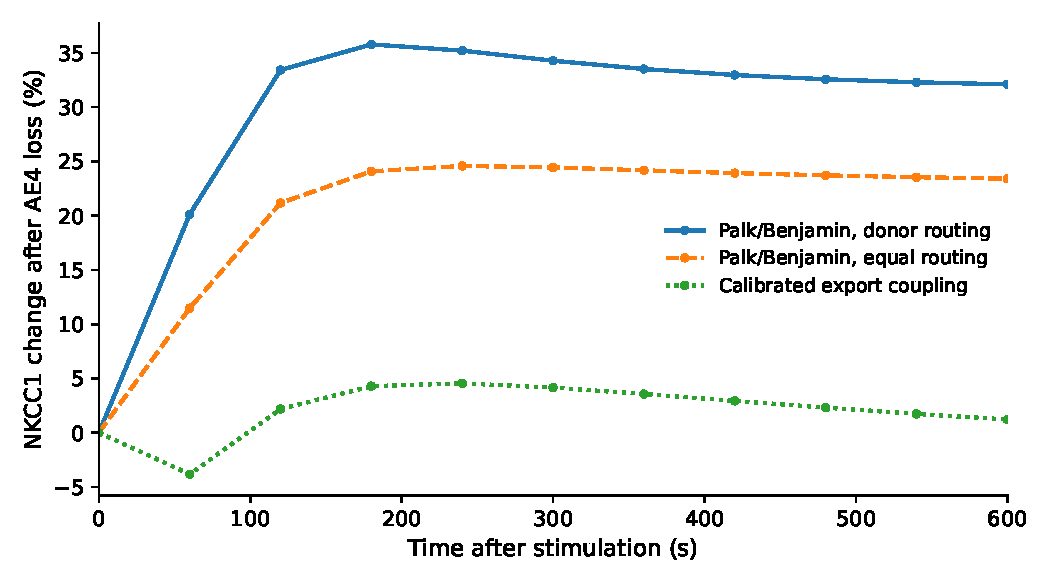
\includegraphics[width=\textwidth]{figures/fig02_nkcc_compensation.pdf}
\caption{Instantaneous NKCC1 chloride flux change after complete AE4 removal, $100(J_N^{\rm KO}/J_N^{\rm WT}-1)$, in three historical reconstructions. Each curve uses its own corresponding wild type and saved 60 s grid. These pointwise ratios are distinct from the reported integrated compensation values and do not simulate the experimental isolated NKCC assay. The export coupling is phenotype calibrated.}
\label{fig:nkcc-compensation}
\end{figure}

\subsection{Molecularly motivated source classes do not by themselves resolve the whole cell mechanism}
\label{sec:catalan-results}

The seven source classes in \cref{tab:mechanism-classes} passed source charge checks and admitted a resting wild type solution. Their predictions were fixed before the phenotype comparison. Eighteen of the 21 genotype trajectories passed the declared checks; the wild type carbonate classes C2, C4a and C4b instead crossed the lower pH limit at approximately 190, 222 and 317 s. Their saved traces end at the recorded failure in \cref{fig:class-ph}. A valid resting solution was not sufficient for physiological secretion.

Among classes with an admissible wild type reference, C1 predicted a 10.76\% \emph{increase} in knockout secretion and a 95.48\% increase in NKCC chloride loading. C3a predicted a 0.72\% secretion increase. The largest valid reduction was 7.67\% in C3b, whose proposed forward affinity was opposed at the reference state. These outcomes are summarised in \cref{tab:class-outcomes}; no failed wild type was replaced by an artificial 600 s endpoint.

\begin{table}[t]
\centering
\caption{Historical source-class outcomes with the inherited scalar kinetic law. Positive deficits mean less knockout fluid; negative values mean more. An absent endpoint is a physiological failure, not a prediction of zero secretion.}
\label{tab:class-outcomes}
\begin{tabularx}{\textwidth}{l r X}
\toprule
Class & Null deficit (\%) & Qualification\\
\midrule
C0 & 3.86 & Equal routing comparator; reference affinity opposed.\\
C1 & $-10.76$ & Valid trajectory; strong compensating NKCC response.\\
C2 & --- & Wild type pH failure at approximately 190 s.\\
C3a & $-0.72$ & Valid trajectory; little genotype separation.\\
C3b & 7.67 & Valid trajectory; reference affinity opposed.\\
C4a & --- & Wild type pH failure at approximately 222 s.\\
C4b & --- & Wild type pH failure at approximately 317 s.\\
\bottomrule
\end{tabularx}
\end{table}

This does not falsify the molecular transport mechanisms proposed by \citet{Catalan2025}. Each test changed the transported source coefficients while retaining an inherited scalar law. Where the new cycle affinity and that law disagree, the construction is not a fully thermodynamically matched kinetic model of the proposed mechanism. The defensible conclusion is that source-vector replacement alone did not produce a substantial, physiologically admissible deficit in this network. Carbonate removal also exposed the importance of distinguishing one carbon atom from two alkalinity equivalents.

\begin{figure}[t]
\centering
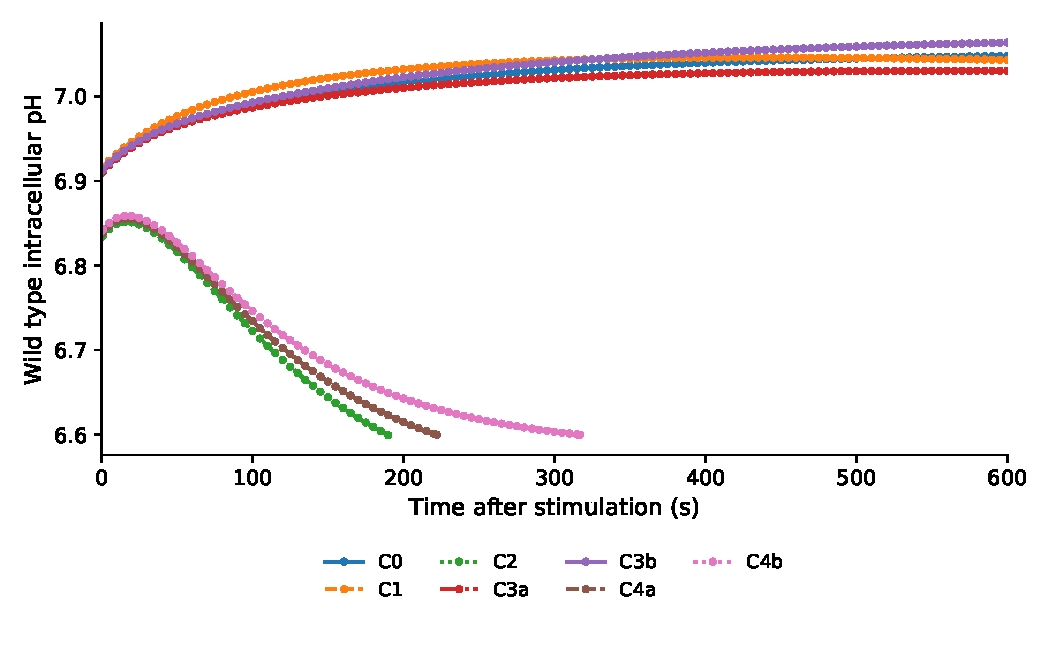
\includegraphics[width=\textwidth]{figures/fig03_class_ph.pdf}
\caption{Recorded wild type pH trajectories for the seven source classes. Curves use the stored samples and stop at their actual endpoints. C2, C4a and C4b reach the lower physiological gate near pH 6.6 before 600 s; the other four classes complete the protocol. Charge neutrality and a resting solution do not prevent a later acid--base failure.}
\label{fig:class-ph}
\end{figure}

\subsection{An effective apical coupling establishes sufficiency, not molecular necessity}
\label{sec:calibrated-coupling}

A separate inverse construction reduced stimulated apical chloride conductance as AE4 expression decreased. Its compact beta conditioned form is
\begin{equation}
 G_{Cl}^{\rm eff}=G_{Cl}^{\rm parent}
 \bigl[1-\lambda a_{Ca}\beta(1-e_4)\bigr],
 \qquad \lambda=0.89488127156712.
 \label{eq:calibrated-coupling}
\end{equation}
Here $a_{Ca}$ is the existing normalised calcium activation and $e_4$ is AE4 expression. Wild type, zero beta input and the resting increment retain their parent vector fields. The coefficient is inherited from phenotype calibration, not measured channel biology. The combined-protocol results are reused from the frozen accepted benchmark with the documented numerical equivalence qualification for coefficient rounding; they are not new integrations.

At full activation, knockout conductance is approximately 10.51\% of its parent value. This strong interaction yields a 30.261\% cumulative null deficit and a 23.163\% deficit at 5\% AE4 expression, while passing the declared 600 s checks. Integrated NKCC compensation falls to approximately 2.79\% in the null. The construction proves that a network interaction can generate a large deficit without eliminating other transporters. It does not prove direct AE4 regulation of TMEM16A, distinguish channel trafficking from another effective interaction, or establish that such a multiplier is required by all alternative explanations.

The temporal comparison in \cref{fig:cumulative-deficits} separates this calibrated benchmark from the small deficit of the compensating model and the final reservoir result. No experimental 600 s percentage is drawn as a band over every earlier time. The trajectory shapes are predictions of their respective assumptions, not fits to minute specific observations.

\begin{figure}[t]
\centering
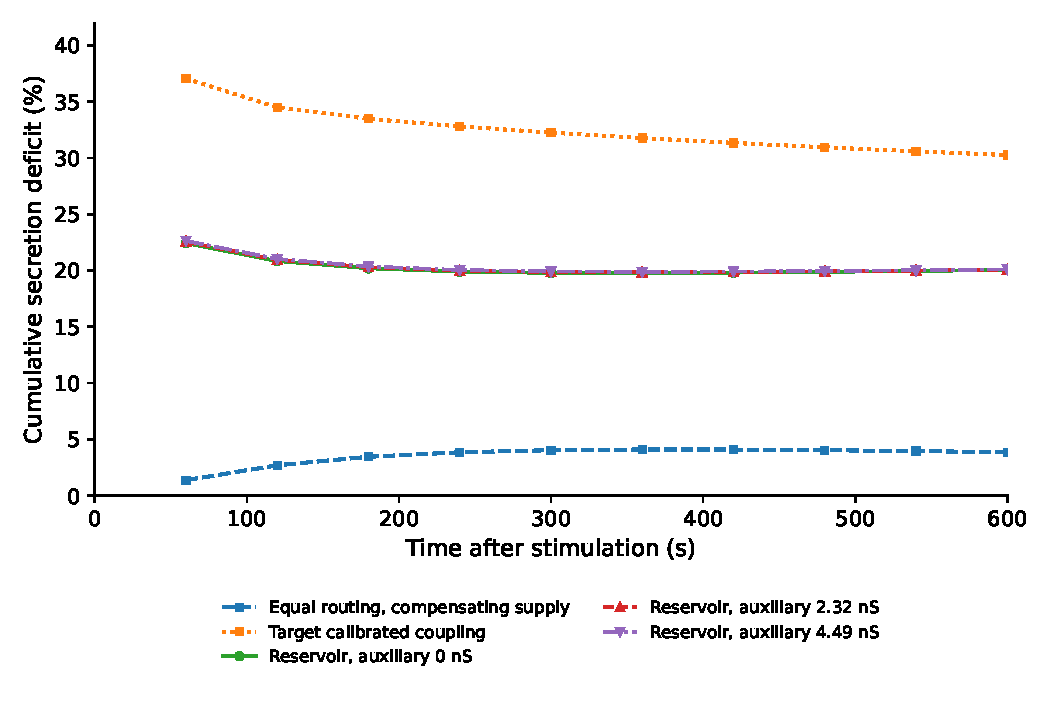
\includegraphics[width=\textwidth]{figures/fig04_cumulative_deficits.pdf}
\caption{Cumulative fluid deficit, $100[1-Q_{\rm KO}(t)/Q_{\rm WT}(t)]$, at the ten declared observation times. The compensating equal routing model gives a small effect; the target calibrated apical coupling gives a larger one. The three final reservoir curves nearly coincide despite different shared auxiliary conductances. Each construction uses its own corresponding wild type. Joining lines connect recorded integral summaries, not newly fitted trajectories.}
\label{fig:cumulative-deficits}
\end{figure}

\subsection{Shared secretory demand reveals the chloride availability difference}
\label{sec:reservoir-result}

The final paired comparison produces a substantial secretion difference without \cref{eq:calibrated-coupling}. All three central cases reach 600 s and pass their frozen sampled physical and conservation checks. Cumulative fluid deficits are 20.039\%, 20.076\% and 20.102\% for auxiliary conductances 0, 2.32 and 4.49 nS, respectively. The range across these alternatives is only 0.062 percentage points. Thus this particular conductance choice is not creating the genotype separation.

At 2.32 nS, wild type secretes 0.978612 pL and knockout 0.782148 pL over 600 s. The mean-flow deficit over 60--600 s is 19.788\%, and the endpoint flow deficit is 20.899\%. The cumulative difference is therefore not a brief effect selected at a favourable observation time. The absolute flow traces are shown in \cref{fig:fluid-flow}; their early transient is not independently calibrated to experimental timing.

\begin{table}[t]
\centering
\caption{Verified central paired outcomes over 0--600 s. Fluid and apical chloride totals use the original headline trapezoidal rule. These are model cell outputs, not absolute whole gland volumes.}
\label{tab:central-results}
\begin{tabular}{rrrrr}
\toprule
$G_{\rm aux}$ & WT fluid & KO fluid & Fluid deficit & Cl export deficit\\
(nS) & (pL) & (pL) & (\%) & (\%)\\
\midrule
0 & 0.972955 & 0.777980 & 20.039 & 18.208\\
2.32 & 0.978612 & 0.782148 & 20.076 & 18.232\\
4.49 & 0.982744 & 0.785197 & 20.102 & 18.249\\
\bottomrule
\end{tabular}
\end{table}

\begin{figure}[t]
\centering
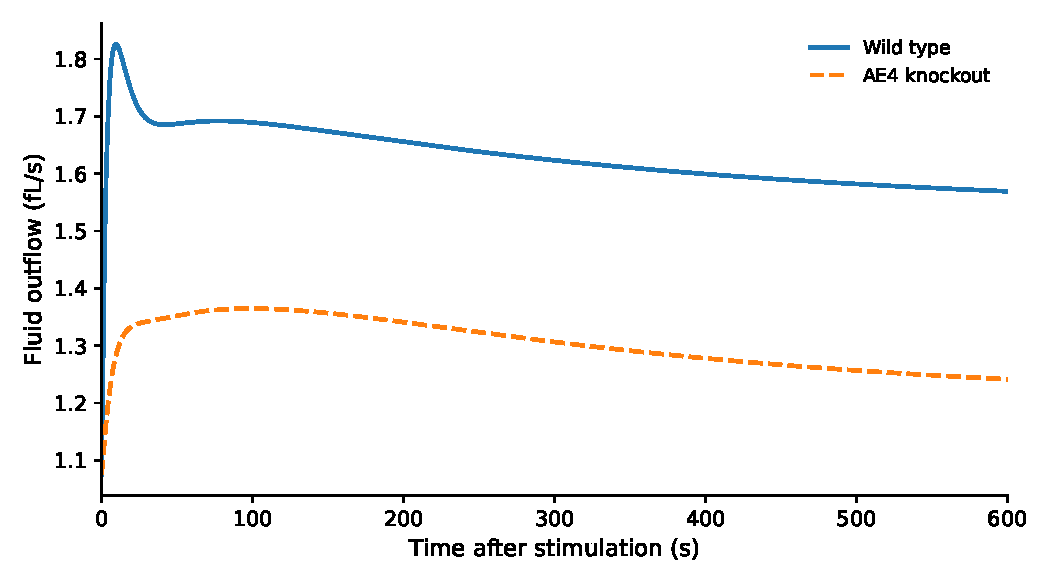
\includegraphics[width=\textwidth]{figures/fig05_fluid_flow.pdf}
\caption{Fluid outflow for the central 2.32 nS shared auxiliary conductance. The knockout has lower flow over the sustained response despite identical prescribed NKCC1 and AE2 supply and identical channel parameters. The curves use saved accepted-step and integer-second samples, including the separate onset convention.}
\label{fig:fluid-flow}
\end{figure}

Wild type retains a larger intracellular chloride concentration throughout the recorded response (\cref{fig:chloride}). Both concentrations initially rise before declining; the mechanism is not complete exhaustion of a fixed chloride store. Wild type continues to load chloride through AE4 while the knockout cannot. At 600 s the central concentrations are approximately 53.71 and 37.50 mM. The associated pH values are 7.029 and 7.274. These later states are predictions conditional on the projection and supply construction, not imposed measurements.

\begin{figure}[t]
\centering
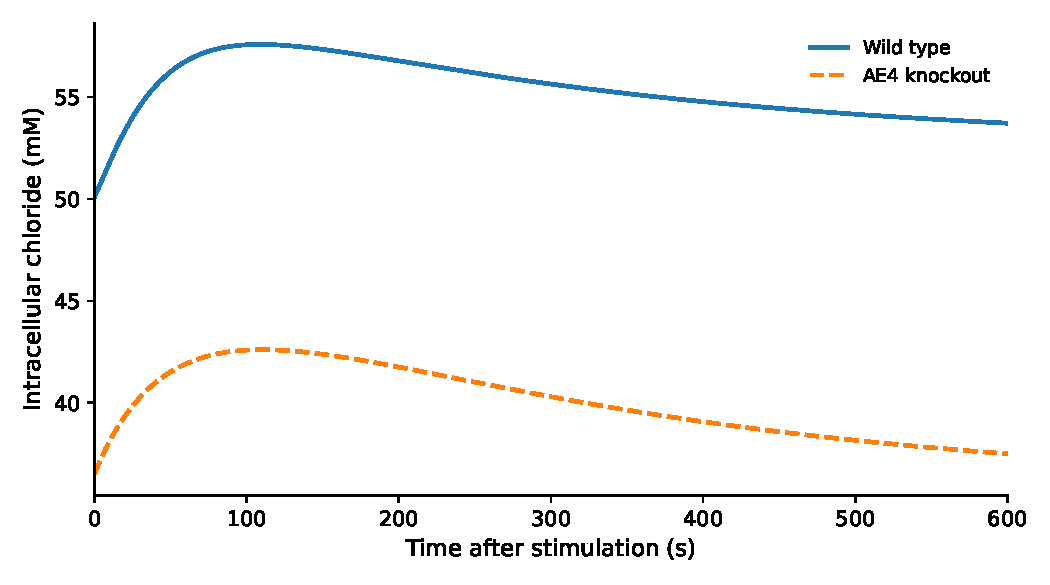
\includegraphics[width=\textwidth]{figures/fig06_chloride.pdf}
\caption{Intracellular chloride in the same central pair. Only the onset chloride values are imposed from the genotype measurements. The subsequent rise and decline are recorded model dynamics. The persistent difference accompanies continuing wild type AE4 supply; it should not be interpreted as simple emptying of the initial store.}
\label{fig:chloride}
\end{figure}

\subsection{The conserved budget accounts for the additional wild type export}
\label{sec:budget-result}

For the central 2.32 nS case, the initial wild type chloride advantage is 19.698595 fmol. Continuing AE4 input contributes another 46.652418 fmol, and 24.487456 fmol of intracellular difference remains at 600 s. Equation~\eqref{eq:reservoir-matched} therefore accounts for 41.863556 fmol of extra wild type apical export. Differential NKCC1 and AE2 contributions are exactly zero by construction. The numerical reconstruction and the independently integrated export are indistinguishable at the figure scale in \cref{fig:reservoir-budget}.

\begin{table}[t]
\centering
\caption{Independent chloride budget using saved Gauss quadrature, including the separately recorded onset term. All amounts are fmol. The two matched non-AE4 supply differences are zero. The last column is the absolute endpoint error in \cref{eq:reservoir-matched}, not an error inferred from the coarse plotting grid.}
\label{tab:budget}
\begin{tabular}{rrrrrr}
\toprule
$G_{\rm aux}$ (nS) & $\delta(0)$ & $D_4$ & $\delta(600)$ & $D_{Cl,a}$ & Error\\
\midrule
0 & 19.698595 & 46.636713 & 24.735190 & 41.600118 & $6.87\times10^{-8}$\\
2.32 & 19.698595 & 46.652418 & 24.487456 & 41.863556 & $7.23\times10^{-8}$\\
4.49 & 19.698595 & 46.663679 & 24.307622 & 42.054652 & $7.49\times10^{-8}$\\
\bottomrule
\end{tabular}
\end{table}

\begin{figure}[t]
\centering
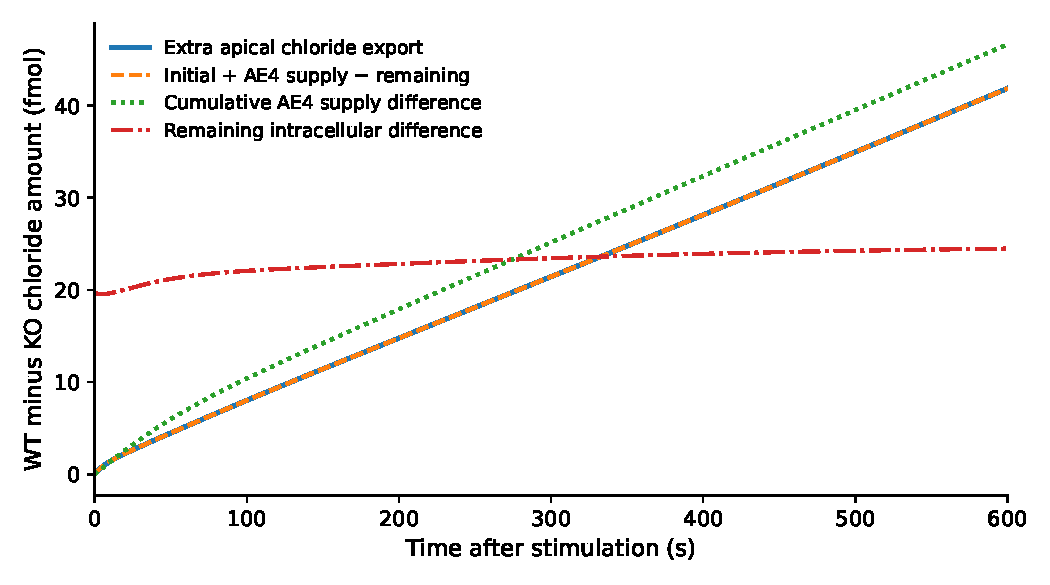
\includegraphics[width=\textwidth]{figures/fig07_reservoir_budget.pdf}
\caption{Time resolved chloride accounting for the central pair. The independently saved extra apical export overlays its mass balance reconstruction, $\delta(0)+D_4(t)-\delta(t)$. The other curves show cumulative AE4 supply and the remaining intracellular difference. Values use the original accepted-step Gauss integrals plus the documented onset contribution; no flux integral is inferred from the state difference.}
\label{fig:reservoir-budget}
\end{figure}

The endpoint errors across all three cases are below $7.5\times10^{-8}$ fmol, compared with the predeclared $10^{-5}$ fmol tolerance. The central headline chloride export deficit is approximately 18.23\%, while its fluid deficit is 20.08\%. Their difference is expected: apical export, net chloride outflow and water outflow are different observables. Exact chloride accounting establishes how much substrate is available to the secretory route, not a universal fixed conversion from exported chloride to fluid volume.

The shared conductance has a smaller driving force in knockout (\cref{fig:driving-force}). At 600 s, the central outward chloride driving forces are approximately 2.03 mV in wild type and 1.60 mV in knockout. Thus equal channel parameters need not give equal chloride currents. This supplies the physical connection between a shared demand pathway and genotype dependent output without an AE4 specific conductance coefficient.

\begin{figure}[t]
\centering
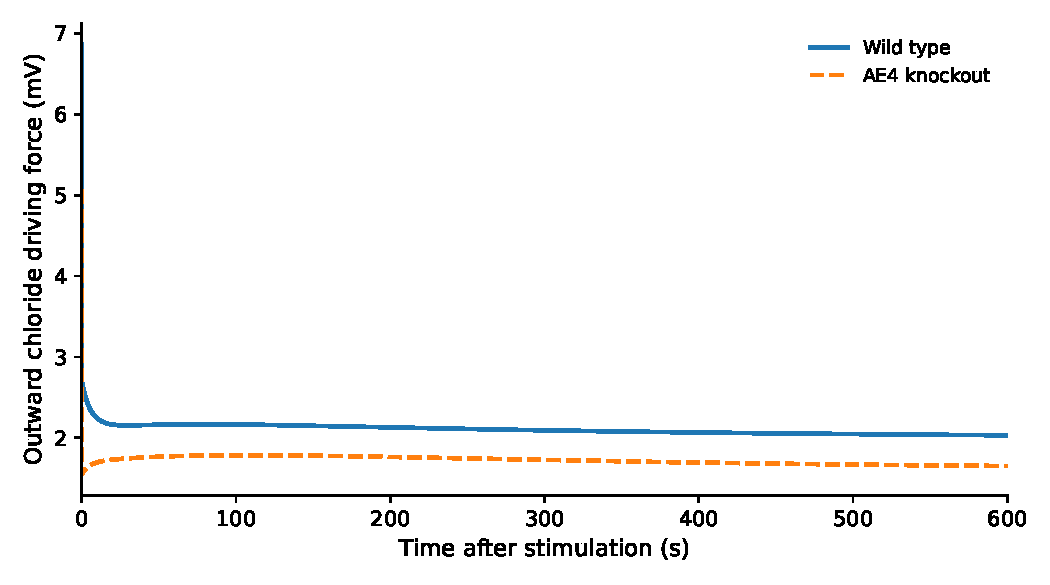
\includegraphics[width=\textwidth]{figures/fig08_driving_force.pdf}
\caption{Outward chloride driving force, $E_{\rm Cl}-V_a$, for the central pair. Identical conductance parameters act on different evolving electrochemical states. The early jump follows the prescribed stimulus convention and is not a fitted experimental onset.}
\label{fig:driving-force}
\end{figure}

\subsection{Reported sensitivities delimit the interpretation}
\label{sec:reported-sensitivities}

The manuscript continuation record reports the outcomes in \cref{tab:reported-sensitivities}. Increasing knockout non-AE4 supply by 5\% or 10\% attenuated, rather than reversed, the deficit. An alternate onset projection gave a similar central magnitude. However, the CCh only result retained much of the effect, and the IPR only trajectory failed the frozen knockout pH check before 600 s. These outcomes are useful qualifications, but their underlying arrays were not available for the independent file checks performed in this manuscript revision. They are deliberately not drawn as time series.

\begin{table}[t]
\centering
\caption{Reported continuation summaries, not independently reverified trajectories in this revision. Values are approximate as preserved in the manuscript decision record. The IPR failure has no valid 600 s secretion endpoint.}
\label{tab:reported-sensitivities}
\begin{tabularx}{\textwidth}{l r X}
\toprule
Comparison & Fluid deficit (\%) & Interpretation of reported outcome\\
\midrule
KO non-AE4 supply $\times1.05$ & 17.65 & Added supply attenuates the effect.\\
KO non-AE4 supply $\times1.10$ & 15.30 & Direction retained under the larger perturbation.\\
Alternate onset projection & 19.77 & Similar magnitude with a different projected state.\\
CCh only & 18.92 & Beta specificity is not established.\\
IPR only & --- & KO pH gate reached at approximately 488 s.\\
\bottomrule
\end{tabularx}
\end{table}

\subsection{Comparison with the original explanation}

The original model, the later compensating network, the calibrated interaction and the reservoir comparison answer different questions (\cref{tab:model-comparison}). The final comparison does not recover the original sodium/pump explanation unchanged. It demonstrates instead that a substantial chloride availability difference can be expressed through otherwise shared secretory pathways. That conclusion is conditional on the projected state and prescribed supply. The conserved accounting is exact; the biological identification of those assumptions is not.

\begin{table}[t]
\centering
\caption{What the main model comparisons establish. Scalar outcomes are kept in a table because no original-model time series is manufactured for this revision. Percentages are not interchangeable fractions of the same mechanism.}
\label{tab:model-comparison}
\begin{tabularx}{\textwidth}{p{0.23\textwidth}rX}
\toprule
Construction & Null deficit & Scientific status\\
\midrule
Original 2018 model & $\sim24\%$ & Cation coupled explanation in the original acid--base and transport network.\\
Later Palk/Benjamin, donor routing & $0.63\%$ & Strong state dependent NKCC compensation.\\
Later equal routing & $3.86\%$ & Small effect despite appreciable WT AE4 loading.\\
Calibrated apical interaction & $30.26\%$ & Proof of sufficiency with a phenotype selected coefficient.\\
Final chloride availability comparison & $20.04$--$20.10\%$ & Conditional mechanism with measured onset constraints and prescribed matched supply.\\
\bottomrule
\end{tabularx}
\end{table}

\section{Discussion}
\label{sec:discussion}

\subsection{AE4 supplies chloride; secretory pathways expose its availability}

The principal result is a conditional mechanism with an explicit mass balance. Wild type begins with more intracellular chloride and retains AE4 mediated chloride loading. When the two genotypes receive matched non-AE4 supply and share apical conductance parameters, knockout exports less chloride and secretes less fluid. A substantial, persistent deficit therefore does not require an AE4 specific apical multiplier in this construction. The reservoir identity accounts for the additional export without invoking an unmeasured source of chloride.

This is stronger than a verbal claim that AE4 maintains a chloride store, but narrower than a complete causal identification of the native knockout phenotype. The initial state is projected using measured chloride and pH, not obtained as a chronic genotype equilibrium. Matched supply is prescribed, not derived from transporter regulation. Projected TIC and potassium differ between genotypes, so the experiment is not an isolated manipulation of chloride alone. The result establishes sufficiency of a particular chloride availability construction within the conserved network, while leaving its biological parameterisation open.

The distinction between a reservoir and a finite store is also important. The model does not empty the entire initial wild type advantage. That difference is larger at 600 s than at onset, and AE4 has supplied additional chloride throughout the interval. The correct explanation is continuing replenishment together with differential availability, not an initial packet of chloride that is simply spent until exhaustion.

\subsection{What changed since the original model}

Our 2018 article provided a plausible network explanation for the striking AE4/AE2 distinction \citep{VeraSiguenza2018}. Its cation dependent AE4 cycle altered intracellular sodium, potassium, NHE1 and pump activity, and predicted weak NKCC activation after exchanger deletion. It should not retrospectively be described as the strongly compensating model: that behaviour emerged in later reconstructions with different transport laws and state responses.

The present analysis changes the evidential status of the explanation rather than negating the original biological observation. The original concentration formulation contained acid--base chemistry, but a successful secretion trace alone did not identify whether sustained alkalinity supply and the partition of transporter fluxes were biologically correct. The amount formulation makes those requirements easier to test. It also exposes that replacing a constitutive law can change the apparent role of AE4 even when the conservation equations and transported stoichiometry remain correct.

The final comparison addresses a further difference. Acute removal at a common wild type state and secretion from established knockout cells are not the same perturbation. A common onset deliberately removes the measured genotype chloride difference. Conversely, imposing that difference does not explain how chronic knockout cells acquired or maintained it. Neither comparison should silently be substituted for the other. Their contrast identifies the need for a future independently constrained account of chronic state formation, not a licence to tune resting conditions against the secretion endpoint.

\subsection{The pitfalls that changed the mechanistic interpretation}
\label{sec:pitfalls}

\paragraph{Conservation is necessary, but not a sufficient biological test.}
An electroneutral source can still drive pH outside the physiological domain. Carbon dioxide transport supplies carbon without net alkalinity, bicarbonate contributes one equivalent of each, and carbonate contributes one carbon but two alkalinity equivalents. Conflating these quantities can make an apparent chloride supply look sustainable when its acid--base budget is not. In the frozen reconstruction, an NBC-like input supplies the additional alkalinity needed for substantial productive AE4 flux. The appropriate inference is conditional on that architecture and its allowed fluxes, not universal necessity of a named transporter. Similarly, a passing 600 s numerical check does not rule out slow modes or later failure.

\paragraph{A plausible compensating law can conceal the phenotype.}
The Palk/Benjamin reconstruction allows changes in intracellular substrates after AE4 removal to raise NKCC chloride uptake substantially. Within that model the compensation is real; the mistake would be to treat the mathematical response as experimentally established merely because the rate law is familiar. The isolated NKCC experiment found no detectable genotype difference under a specific depletion and readdition protocol \citep{Pena2015}. Its conditions are not normal whole cell stimulation, and the reduced Palk law does not reproduce the external substrate manipulation faithfully. Thus neither the large simulated compensation nor exact equality of physiological fluxes is proved by that assay. The final matched-supply comparison is useful precisely because it makes the alternative assumption explicit.

\paragraph{An algebraic cancellation is not zero biological sensitivity.}
Equation~\eqref{eq:equal-routing-identity} removes the explicit AE4 term for equal routing, but AE4 can change pump and NHE1 activity through the state. The identity does not make secretion independent of AE4, nor does it identify a globally optimal intervention or a universal minimum coupling strength. Its value is diagnostic: it explains why searching source coefficients alone may fail to control sustained export. The chloride identity in \cref{eq:reservoir-general} avoids this routing restriction and remains useful for finite time comparisons.

\paragraph{Source stoichiometry and a kinetic law are different commitments.}
A proposed cycle can pass charge accounting while an inherited scalar law drives it against its own affinity. The seven-class panel therefore tests a specified source replacement, not every possible kinetic realisation of the molecular proposal. Its physiological failures and small or reversed deficits are informative exclusions within that construction. They cannot be promoted to a refutation of the biochemical measurements. Full consistency would require class specific kinetics with compatible reversal, substrate dependence and capacity, constrained independently of secretion.

\paragraph{Opening a volume sensitive pathway requires an initiating perturbation.}
The earlier swelling-only VRAC construction attached a positive swelling gate to an AE4 knockout core with no beta driven upstream change. At an exact unchanged resting state, such a gate cannot initiate its own activating perturbation. This excludes that circular initiation mechanism, not every role of volume sensitive channels. Adding beta driven NKCC loading changes the premise and permits local chloride loading and swelling. However, local initiation does not identify the conductance needed for sustained secretion.

The subsequent independently targeted swelling calculation illustrates the distinction. At the two frozen conductance endpoints, mean swelling was approximately 5.75\% and 2.44\%, rather than the prescribed 12.5\% target. The residuals did not bracket a root, so no accepted conductance or quantitative beta-protocol prediction followed. Two endpoints do not prove global absence of a solution or monotonicity. The scientifically useful result is the unresolved identification, retained without extra searches or phenotype based rescue.

\paragraph{Calibrated sufficiency must not become an inferred molecular mechanism.}
Equation~\eqref{eq:calibrated-coupling} demonstrates that an added interaction can generate a large deficit, but its coefficient derives from the phenotype. Agreement is therefore not an independent validation. The final reservoir result shows that such a multiplier is not required for a substantial deficit in the stated alternative construction. Conversely, it does not exclude additional beta conditioned interactions in the gland. The two models are not additive components, and their percentage effects cannot be summed or subtracted to estimate an unobserved pathway.

\subsection{Catalán 2015: a shared demand pathway, not necessarily an AE4 specific channel}

The 2015 TMEM16A deletion experiment separates muscarinic calcium dependent secretion from an IPR responsive route \citep{Catalan2015}. Persistence of the latter, its swelling association and sensitivity to DCPIB/NPPB support considering an auxiliary anion pathway. They do not establish a direct AE4-to-channel interaction or a unique molecular channel identity. Our shared auxiliary conductance is an effective representation of demand, not a claim that the entire measured whole cell current is apical or that its conductance follows directly from a holding voltage.

The final model permits a different location for the genotype dependence: substrate availability rather than channel abundance. Identical conductance parameters act on different chloride concentrations and membrane potentials, so their currents differ. The modest effect of varying auxiliary strength on the relative deficit indicates that the shared pathway is not the adjustable source of the phenotype in this comparison. Indeed, a similar deficit persists when the added conductance is zero. This supports chloride availability as a general secretory constraint but does not explain the experimental selectivity of beta containing uptake responses.

\subsection{Catalán 2025: molecular constraints do not uniquely fix a gland model}

The human AE4 mutagenesis and molecular dynamics results identify a putative region coordinating cations and bicarbonate around the TM3--TM10 interface \citep{Catalan2025}. The different sodium and potassium responses of the T448I/T756A double mutant are especially important: cation participation is not a dispensable label on an otherwise specified chloride exchanger. Nevertheless, coordination and mutant activity do not uniquely determine whole-cycle stoichiometry, the sodium/potassium flux split at native concentrations, or the kinetic response during salivary stimulation.

The original concentration weighted allocation, the later equal allocation and the final retained donor allocation are therefore effective model choices, not rival direct measurements of the protein. Our source-class panel makes part of that uncertainty explicit, while also demonstrating the danger of combining a proposed source vector with an unchanged kinetic law. The reservoir identity does not resolve the molecular cycle; it provides a conservation constraint that any admissible cycle must satisfy once its actual chloride input has been specified. This is the useful connection between the molecular study and the present article: molecular evidence constrains possible transport, whereas the full cell budget determines how that transport can influence secretion.

\subsection{Why approximately 35\% is context rather than a mathematical constant}

The experimental deficit is an observation with sampling uncertainty, protocol dependence and a different spatial scale from a single model cell. The reported standard error is not a confidence bound and cannot define an acceptance threshold by subtraction from the mean. A 20\% conditional prediction is not automatically a failure because it differs from 35\%, just as a fitted 35\% result is not automatically validated.

The relevant achievement is a substantial reduction of the correct direction, persisting across the declared observation windows without selection of an AE4 specific channel coefficient against that outcome. The relevant remaining weaknesses are mechanistic: imposed onset states, matched supply, unmeasured projected quantities and incomplete stimulus specificity. It would be equally unjustified to claim that the model explains $20/35$ of the biological mechanism or that the numerical difference identifies a missing 15 percentage point pathway. Different constructions, observation maps and baselines do not support that arithmetic as causal attribution.

\subsection{Limitations and discriminating observations}

The source chloride and pH measurements constrain onset, but do not identify all intracellular carbon species, potassium, volume or their covariance. The central projection substantially changes TIC between genotypes. The reported alternate projection is a useful sensitivity, not proof that all admissible onsets agree. Likewise, the reported extra-supply cases suggest attenuation without sign reversal, but cannot replace measurements of non-AE4 fluxes under matched native stimulation. Their original arrays require deposition before those sensitivity claims are fully reproducible from this revision's source package.

The reported CCh only deficit and IPR pH failure remain substantive qualifications. A CCh only fluid deficit cannot be compared directly with preserved SPQ uptake: a fluorescence recovery slope, a concentration derivative and gland fluid output have different observation maps. For example, $\dd[\Cl]_i/\dd t=(\dot n_{\rm Cl,i}-[\Cl]_i\dot V_i)/V_i$ includes dilution. Nevertheless, retention of much of the model deficit without beta stimulation means protocol specificity has not been established. A trajectory that crosses the pH limit near 488 s has no accepted 600 s endpoint, regardless of what its unvalidated continuation might suggest.

No final reservoir AE2 knockout or chronic 5\% AE4 comparison was performed. The original AE2 specificity result and exact nesting properties of the calibrated benchmark must therefore not be transferred to the final construction. The single cell approximation, effective signalling inputs and absent ductal model also limit quantitative interpretation. The strict conservation identity does not remove these biological limitations.

The most discriminating additional observations would separate supply from demand under the same stimulation protocol: genotype specific chloride amounts and cell volume, non-AE4 chloride uptake, pH and bicarbonate handling, and apical current with an identified driving force. Such observations could determine whether compensation is genuinely constrained and whether the measured reservoir difference survives without imposing it. This is a narrower and more informative requirement than adding an unconstrained channel multiplier until one secretion percentage is reproduced.

\subsection{Conclusion}

The experimental importance of AE4 survives the reassessment, but the original cation-routing explanation does not remain uniquely determined. A conservation based model reveals how alkalinity supply enables chloride loading, how compensating transport can conceal AE4 loss, and how plausible channel or source constructions can fail physiological or identification tests. Under explicit onset and matched-supply assumptions, a larger chloride reservoir together with continuing AE4 input gives wild type a sustained export advantage through shared secretory pathways. The result provides partial mechanistic support for chloride availability as a basis of AE4 dependent secretion. Its strengths are the substantial conditional effect and exact mass accounting; its unresolved parts are chronic state formation, native compensation and stimulus specificity.


\section*{Data and code availability}
The public repository \url{https://github.com/esig626/ae4-salivary-transport-control} contains the model lineage, frozen central trajectories and historical comparisons. This revision uses the scientific source snapshot \nolinkurl{764e32a648ee3b69265364788df5a59f76cb2843}; no model was rerun for the article. The eight figures are regenerated by \nolinkurl{manuscript/scripts/build_figures.py}. Plotting tables, input SHA256 hashes and arithmetic checks are supplied in \nolinkurl{manuscript/data/time_series/}, with PDF and EPS figures in \nolinkurl{manuscript/figures/}.

The additional supply, projection and single agonist outcomes in \cref{tab:reported-sensitivities} are preserved as reported continuation summaries in the manuscript decision record. Their underlying trajectories were not present in the source snapshot used for this revision and were not independently rechecked here. They are not used to generate figures or to claim additional validated 600 s trajectories. Deposition of those original files remains necessary for a fully reproducible submission. The verified central result and its complete numerical budget do not depend on treating these reported sensitivities as independently verified data.

\section*{Author contributions}
To be completed after the author list has been agreed.

\section*{Funding}
To be completed before submission.

\section*{Competing interests}
To be confirmed by all authors before submission.

\bibliographystyle{plainnat}
\bibliography{references}

\end{document}
